%!TEX root = ../main.tex

Through convex reformulations, we have characterized the optimal sets of ReLU
networks, computed minimal networks, and provided sensitivity results.
Our goal in this section is to illustrate the power of our framework for
analyzing ReLU networks and developing new algorithms.


\setlength{\tabcolsep}{2.5pt}
\begin{table}[t]
	\centering
	\caption{Tuning neural networks by searching over the optimal set.
		We fit two-layer ReLU networks on the training set and
		compute the minimum \( \ell_2 \) norm solution (Min L$_2$).
		Then we tune by finding an extreme point approximating
		the maximum \( \ell_2 \)-norm solution (EP), minimizing validation
		MSE over the optimal set (V-MSE), and minimizing test MSE over
		the optimal set (T-MSE).
		Results show median test accuracy;
		Max Diff. reports the difference between the best and worse models
		found.
		Exploring the optimal set reveals a huge disparity in the performance
		of optimal networks, with the generalization gap exceeding \( 20 \)
		points on four datasets.
	}
	\label{table:tuning-small}
	\vspace{0.1in}
	\begin{tabular}{lccccc} \toprule
		\textbf{Dataset} & \textbf{Min L$_2$} & \textbf{EP} & \textbf{V-MSE} & \textbf{T-MSE} & \textbf{Max Diff.} \\
		\midrule
		fertility        & 0.66               & 0.69        & 0.65           & 0.64           & 0.05               \\
		heart-hung.      & 0.75               & 0.75        & 0.71           & 0.85           & 0.14               \\
		mammogr.         & 0.77               & 0.77        & 0.57           & 0.78           & 0.21               \\
		monks-1          & 0.67               & 0.66        & 0.49           & 0.57           & 0.17               \\
		planning         & 0.53               & 0.52        & 0.53           & 0.7            & 0.17               \\
		spectf           & 0.64               & 0.64        & 0.56           & 0.58           & 0.08               \\
		horse-colic      & 0.75               & 0.59        & 0.74           & 0.85           & 0.26               \\
		ilpd-indian      & 0.59               & 0.59        & 0.53           & 0.72           & 0.19               \\
		parkinsons       & 0.74               & 0.74        & 0.65           & 0.88           & 0.23               \\
		pima             & 0.68               & 0.68        & 0.68           & 0.87           & 0.2                \\
		\bottomrule
	\end{tabular}
\end{table}


\textbf{Tuning}:
We first consider a tuning task on 10 binary classification
datasets from the UCI repository~\citep{dua2019uci}.
For each dataset, we do a train/validation/test split, fit a two-layer
ReLU model on the training set, and then compute the minimum \( \ell_2 \)-norm
model.
We use this to explore the optimal set in three ways:
(i) we compute an extreme point that (approximately)
maximizes the model's \( \ell_2 \)-norm; (ii)
we minimize the validation MSE over
\( \solfn(\lambda) \); (iii) we minimize test MSE over \( \solfn(\lambda) \).
These procedures select for different optimal models,
have no effect on the training objective, and are only possible
because we know \( \solfn \).

The results are summarized in \cref{table:tuning-small}.
We see that optimal models can perform very differently at test time despite
having exactly the same training error and model norm.
Indeed, 9/10 datasets show at least a 10 percent gap between the best
and worst models and 4/10 have a gap exceeding 20 percent accuracy.
We conclude that the training objective is badly under-determined even for
shallow neural networks, implying that implicit regularization is critical
in practice.
See \cref{app:sol-fn-additional-experiments} for results on additional datasets.

\begin{figure}[t]
    \centering
    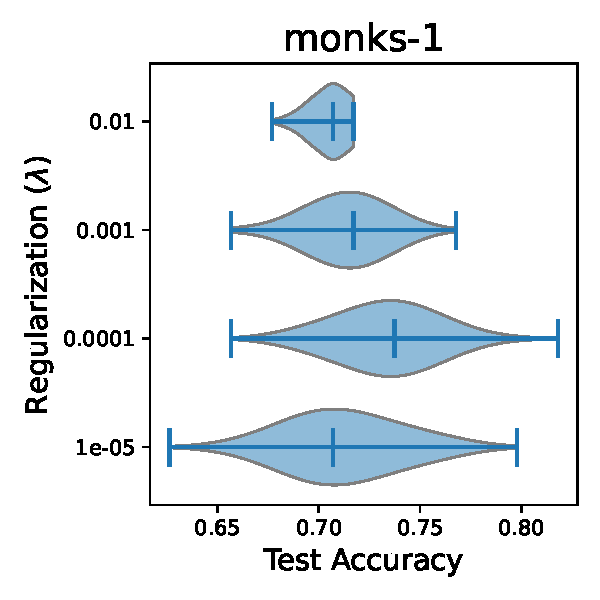
\includegraphics[width=0.48\textwidth]{figures/chapter_three/dist_paper_monks-1.pdf}%
    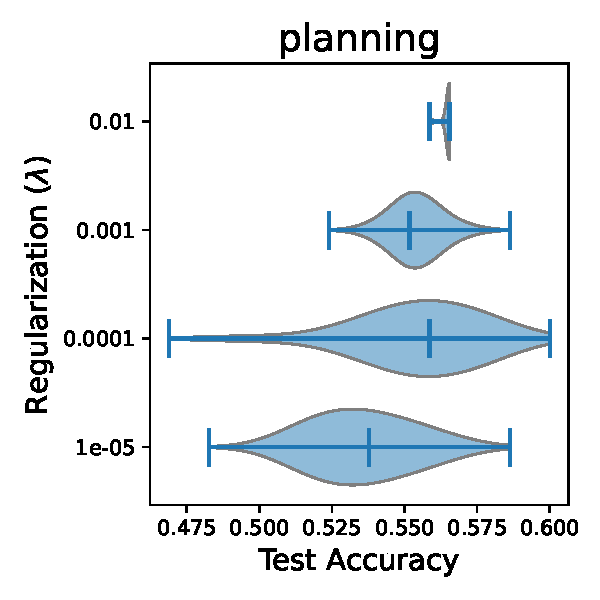
\includegraphics[width=0.48\textwidth]{figures/chapter_three/dist_paper_planning.pdf}
    \caption{Distribution of test accuracy over 10,000 uniform samples taken from
        the optimal sets for two-layer ReLU networks trained on two datasets from
        the UCI repository.
        Generalization performance varies by approximately
        \( 20\% \) when regularization small, with the majority of
        mass concentrated around models of middling performance.
        As expected, increasing the regularization reduces the generalization
        gap between models.
        For both problems, the best test accuracy is achieved by a small
        proportion of models at \( \lambda = 10^{-4} \).}%
    \label{fig:uci-sampling-paper}
\end{figure}

\begin{figure}[t]
    \centering
    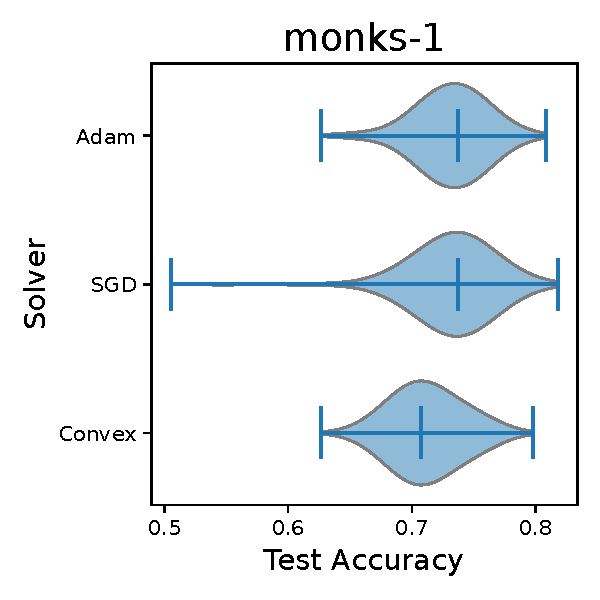
\includegraphics[width=0.48\textwidth]{figures/chapter_three/nc_comparison_monks-1.pdf}%
    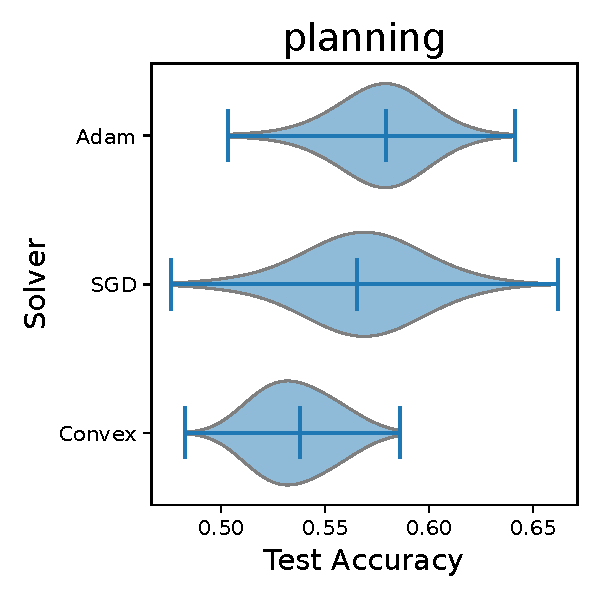
\includegraphics[width=0.48\textwidth]{figures/chapter_three/nc_comparison_planning.pdf}
    \caption{Implicit regularization of SGD and Adam on two datasets from the
        UCI repository with regularization strength \( \lambda = 10^{-5} \).
        Each method is run with \( 1000 \) different random initializations
        in order to approximately sample models from the optimal set.
        To ensure stationarity, we reject any final model where the
        pseudo-gradient norm is larger than \( 10^{-6} \).
        Note that SGD and Adam may converge to local minima, leading to
        different generalization as compared to the true optimal set.
        Surprisingly, we find that the distribution of generalization
        performance for SGD and Adam is quite similar to the ground-truth
        optimal set, particularly for \texttt{monks-1}.
    }%
    \label{fig:uci-optimizer-sampling}
\end{figure}

\textbf{Sampling}:
The previous experiment demonstrates that different optimal models can perform
very differently at test time.
However, selecting models by minimizing or maximizing a specific selection
function only captures a small (measure-zero) part the optimal set and its
generalization behavior.
Hit-and-run samplers \citep{boneh1979constraints, smith1980monte, smith1984efficient}
provide an alternative method of selecting optimal models by generating a
Markov chain which (when sufficiently thinned) yields a
uniform sample over \( \solfn(\lambda) \).

\cref{fig:uci-sampling-paper} shows the distribution of test
accuracy over \( 10,000 \) samples taken from the optimal set using
hit-and-run.
Similar to \cref{table:tuning-small}, we observe a large gap in generalization
performance between the best and worst-performing optimal models.
This gap closes as the regularization strength increases, reflecting how
increased regularization shrinks the optimal set towards zero and decreases
the number of active neurons.

We also compare the implicit regularization of SGD and Adam against the
generalization performance of all global optima.
\cref{fig:uci-optimizer-sampling} shows the distribution of
test accuracy for \( 1000 \) random restarts of SGD and Adam as compared
to the ground-truth distribution obtained using hit-and-run on
the \texttt{monks-1} and \texttt{planning} datasets.
Interestingly, SGD and Adam do not show a strong bias towards solutions with
better test accuracy, suggesting that the effects of implicit regularization
are not strong for two-layer networks on these datasets.
See \cref{app:sol-fn-additional-experiments} for experimental details and
results for additional datasets.

\begin{figure*}[t]
    \centering
    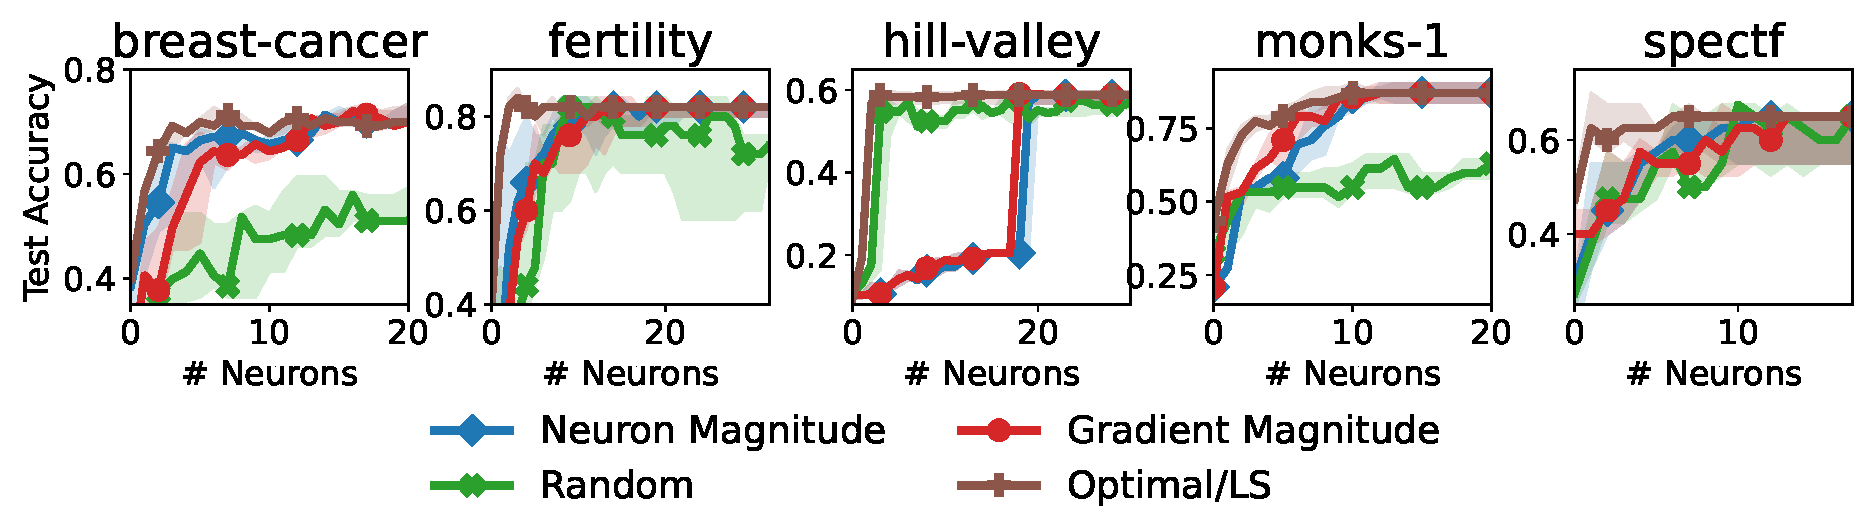
\includegraphics[width=0.98\textwidth]{figures/chapter_three/uci_pruning_acc.pdf}
    \caption{Pruning neurons from two-layer ReLU networks on binary
        classification tasks from the UCI repository.
        We compare our theory-inspired approach (\textbf{Optimal/LS}),
        against removing the neuron with smallest \( \ell_2 \) norm
        (\textbf{Neuron Magnitude}),
        removing the neuron with the smallest weighted gradient norm
        (\textbf{Gradient Magnitude}), and random pruning (\textbf{Random}).
        For Optimal/LS, we use \cref{alg:pruning-solutions-nn}, which begins
        with optimal pruning and then switches to a least-squares heuristic.
        We plot test accuracy against number of active neurons.
        Optimal/LS dominates the baseline methods on every dataset
        and even improves test accuracy on \texttt{breast-cancer}
        and \texttt{fertility}.
    }%
    \label{fig:uci-pruning-acc}
\end{figure*}

\begin{figure}[t]
    \centering
    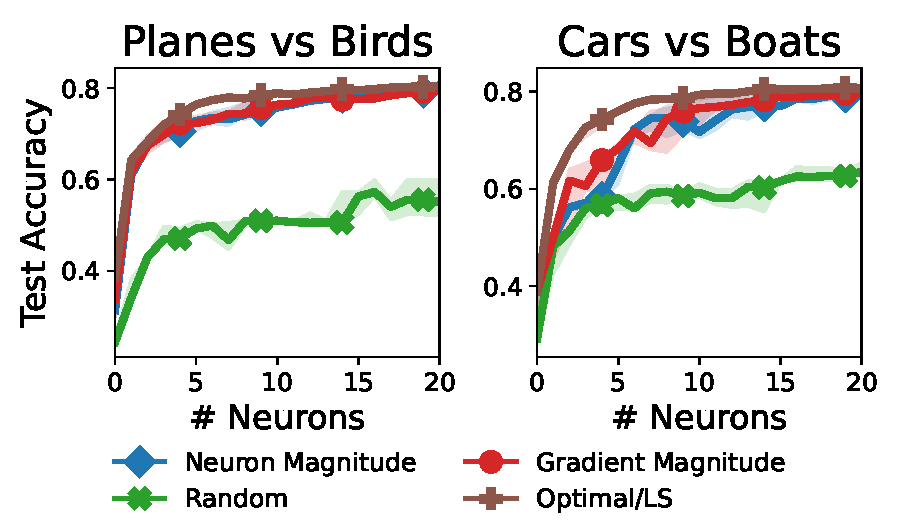
\includegraphics[width=0.98\textwidth]{figures/chapter_three/cifar_pruning_acc.pdf}
    \caption{Pruning neurons from two-layer ReLU networks on two binary
        classification tasks drawn from the CIFAR-10 dataset.
        We compare our method (\textbf{Optimal/LS}) against baselines;
        see \cref{fig:uci-pruning-acc} for details.
        Our approach, which makes use of a weight correction after pruning,
        outperforms every baseline.
    }
    \label{fig:cifar-pruning-acc}
\end{figure}

\textbf{Pruning}:
We also consider several neuron pruning tasks.
We use two-layer ReLU networks and start pruning from the model given
by optimizing the convex reformulation.
We compare four strategies:
(i) pruning neurons optimally using
\cref{alg:pruning-solutions-nn} until \( \cbr{(XW^{(1)}_{\cdot, i})_+}_\act \) are linearly
independent and then approximately using least-squares fits;
and (ii) by removing the neuron with the smallest magnitude,
\( \norm{W^{(1)}_{\cdot, i} \cdot W^{(2)}_{i}} \);
(iii) by removing the neuron with the smallest weighted gradient;
and (iv) by random pruning.

\cref{fig:uci-pruning-acc} shows test performance of the these methods for five
UCI datasets.
Our theory-based pruning method has better test performance
than the baselines on every dataset considered;
on \texttt{hill-valley}, the gap between our approach and
magnitude-based pruning is approximately \( 40\% \).
\cref{fig:cifar-pruning-acc} presents similar results for two binary tasks
taken from the CIFAR-10 dataset \citep{krizhevsky2009learning}.
We provide experiments on additional datasets, including MNIST
\citep{lecun1998gradient},
and experimental details in
\cref{app:sol-fn-additional-experiments}.

